\documentclass[tikz,border=6pt]{standalone}
\usepackage{tikz}
\usetikzlibrary{arrows.meta,positioning}

\begin{document}
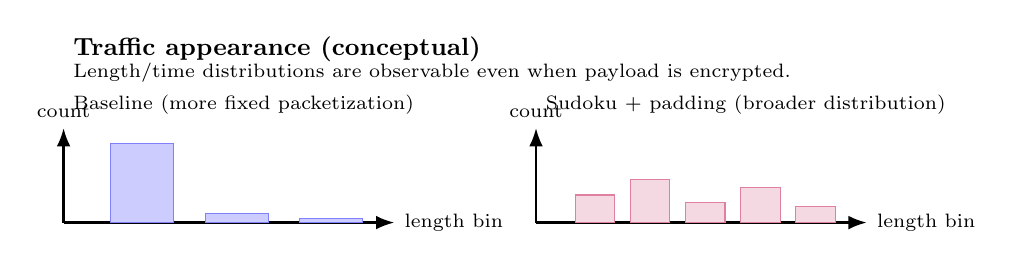
\begin{tikzpicture}[
  font=\small,
  axis/.style={-Latex,thick},
  bar/.style={fill=blue!20,draw=blue!50},
  bar2/.style={fill=purple!15,draw=purple!50},
]
  % Baseline histogram (fixed length)
  \node[font=\small\bfseries,anchor=west] at (0,2.2) {Traffic appearance (conceptual)};
  \node[font=\scriptsize,anchor=west] at (0,1.9) {Length/time distributions are observable even when payload is encrypted.};

  \node[font=\scriptsize,anchor=west] at (0,1.5) {Baseline (more fixed packetization)};
  \draw[axis] (0,0) -- (4.2,0) node[right,font=\scriptsize]{length bin};
  \draw[axis] (0,0) -- (0,1.2) node[above,font=\scriptsize]{count};
  \draw[bar] (0.6,0) rectangle (1.4,1.0);
  \draw[bar] (1.8,0) rectangle (2.6,0.12);
  \draw[bar] (3.0,0) rectangle (3.8,0.05);

  % Sudoku histogram (padding broadens distribution)
  \begin{scope}[xshift=6.0cm]
    \node[font=\scriptsize,anchor=west] at (0,1.5) {Sudoku + padding (broader distribution)};
    \draw[axis] (0,0) -- (4.2,0) node[right,font=\scriptsize]{length bin};
    \draw[axis] (0,0) -- (0,1.2) node[above,font=\scriptsize]{count};
    \draw[bar2] (0.5,0) rectangle (1.0,0.35);
    \draw[bar2] (1.2,0) rectangle (1.7,0.55);
    \draw[bar2] (1.9,0) rectangle (2.4,0.25);
    \draw[bar2] (2.6,0) rectangle (3.1,0.45);
    \draw[bar2] (3.3,0) rectangle (3.8,0.20);
  \end{scope}
\end{tikzpicture}
\end{document}

